\clearpage
\begin{flushright}
	\textit{Лекция №17}
	\textit{2015.11.17}
\end{flushright}

Способ синхронизации – часы. Работают на импульсах тактового генератора. Они имеют точность, поэтому имеют свойство спешить или отставать.
В развитых странах есть служба точного времени.
Интервал между 2 последовательными солнечными переходами называется солнечным днем. В результате измерений была определена солнечная секунда (min solar second). В 1948 году были изобретены атомные часы, обладающие высокой стабильностью, и было определено, что за одну секунду будет совершено 9192631770 переходов цезия133. 50 лабораторий мира имеют такие часы. Международное бюро усредняет эти данные и выдает время по атомным часам. TAI - International Atomic Time.
Средний солнечный день усредняется. Атомная секунда не меняется. Полдень будет наступать раньше, чем реальный полдень. В результате было решено использовать потерянные секунды. Всякий раз, когда разница возрастает до 800мс, то добавляется секунда. Так перешли на UTC. 
Большинство электрических компаний положили в основу это универсальное согласованное время UTC. Когда бюро объявляет потерянную секунду, то частоту герцевых часов меняют с 60->61 или 50->51.
В  США есть институт точного времени. Они имеют коротковолновую станцию. В начале каждой секунды осуществляют рассылку. 

Один комп оборудован приемником WWV, остальные подводятся.
Алгоритмы  синхронизации:
\begin{enumerate}
    \item Cristian’s
    \item Berkeley
    \item усредняющие
\end{enumerate} 

В распределенных системах стоит задача синхронизации. Представим локальную сеть, на каждом компе есть локальное время, но они подводят \ref{pic:trable_sync}.

\begin{figure}[H]
    \centering
    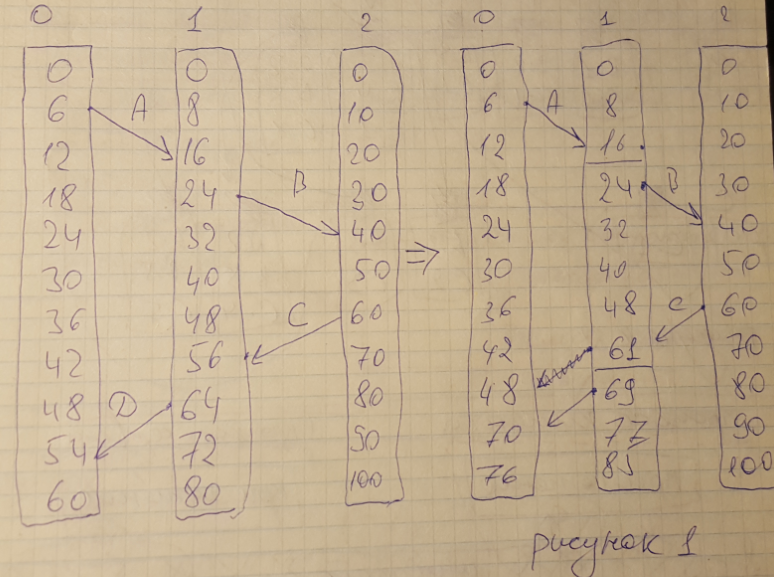
\includegraphics[width=\textwidth]{pic/1.png}
    \caption{pic}
    \label{pic:trable_sync}
\end{figure}

Есть алгоритмы синхронизации по логическим часам. Предложил в 1978 году Лампорт. Должно выполняться соотношение: случилось до – случилось после. Если событие $A$ произошло до события $B$, то $tA < tB$. Это мы гарантировать не можем. Лампорт предложил при взаимодействии параллельных процессов, которые обмениваются сообщениями добавлять в это сообщение время отправки по локальным часам. Процесс, который получает сообщение, смотрит, а какое его локальное время и устанавливает свое время равное времени пришедшего в сообщении + 1, если его время меньше.

Проблема – ситуация, когда время двух событий одинаковое. Возникает неоднозначность.
В 1988 году разработан алгоритм векторные часы. Передаем не просто значения локального счетчика и корректировать собственный локальный счетчик, тут формируется вектор, на \ref{pic:vec_watch} показан процесс передачи сообщений тремя процессами и показано, что для последующего состояния системы состояния B:4 – исходное. Это не время, это событие (посылка и отправка сообщения). Каждое сообщение содержит локальный счетчик.

\begin{figure}[H]
    \centering
    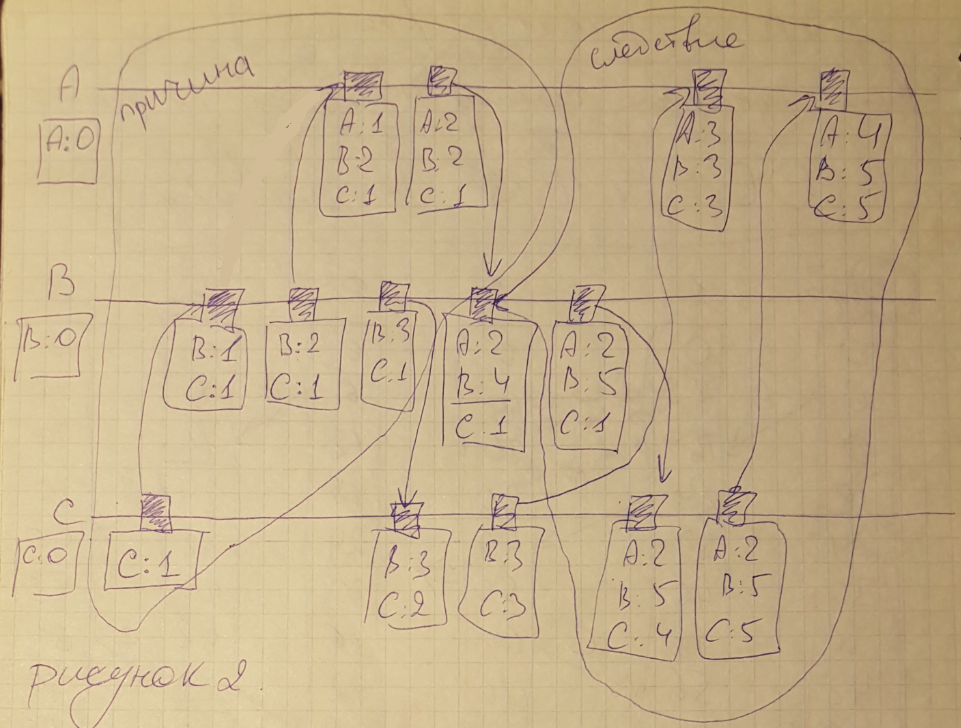
\includegraphics[width=\textwidth]{pic/2.png}
    \caption{алгоритм векторные часы}
    \label{pic:vec_watch}
\end{figure}

В распределенных системах возникает задача разделения ресурсов.

\section{Алгоритмы взаимного исключения}

\subsection{Централизованный алгоритм (забияки)}

с выбором нового координатора. Самый надежный. Предполагает наличие некоторого процесса координатора. Обычно в качестве процесса координатора выбирается процесс, который имеет наибольший сетевой номер. Когда какой-то процесс хочет войти в свою критическую секцию он посылает сообщение запрос координатору, указывая критическую секцию, в которую он хочет войти и ждет от координатора разрешения. Если в этот момент ни один процесс не находится в критической секции, то координатор посылает сообщение разрешение. Если некоторый процесс уже находится в критической секции, то никакой ответ не посылается, а сообщение запрашивающего процесса ставится в очередь. Затем по мере освобождения критической секции просматривается очередь и процессу будет послано сообщение разрешение.   Координатор координирует вход в критическую секцию. Чтобы сохранить работоспособность системы, при обнаружении любым из процессов отсутствие координатора этот процесс инициализирует выборы нового координатор путем посылки сообщения-запроса со своим номером. Если номер процесса получившего сообщение запрос о начале выборов больше, то он посылает назад подтверждение прием и сам инициализирует новые выборы. В результате выполнения такое цепочки действий выбирается новый координатор и им становится процесс с большим сетевым номером. 

\subsection{Распределенный алгоритм}

Когда процесс хочет войти в свой критический участок по конкретному ресурсу он формирует сообщение, в котором указывает идентификатор критической секции, свой номер и своё локальное время. Это сообщение посылается остальным процессам. При этом предполагается, что получение такого сообщение надежно, оно подтверждается получением сообщения. Когда процесс получает такое сообщение запрос, его действия зависят от того, в каком состоянии относительно критической секции он сам находится. 

Допустимы три ситуации:
\begin{enumerate}
    \item процесс получивший сообщение не находится и не собирается входить в данную критическую секцию, тогда он посылает процессу, приславшему сообщение, ответ с разрешением;
    \item процесс, получивший сообщение, уже находится в критической секции по данному ресурсу. В этом случае он не посылает ничего и ставит это сообщение в очередь;
    \item процесс, получивший сообщение сам хочет войти в данную критическую секцию, тогда он сравнивает временную отметку в полученном сообщении с временной отметкой его собственного сообщения. Если время поступившего к нему сообщения меньше его собственного времени (его запрос возник позже) то он посылает сообщение разрешение, иначе ничего не посылает и ставит пришедшее сообщение в очередь.
\end{enumerate} 

Процесс может войти в критическую секцию, если получит N-1 сообщение-разрешение от других процессов. Если любой из процессов завершился, то уже не получить N-1 сообщение.

\subsection{Алгоритм Token ring}

Формируется логическое кольцо, в котором каждый процесс знает номер своих соседей. 1984 год фирма IBM. Token – специальное сообщение, которое создается для конкретной критической секции. Такой token циркулирует по кольцу.  Когда процесс получает  token от своего соседа, он анализирует, не требуется ли ему войти в данную критическую секцию, если нет – он сразу посылает token дальше, если ему нужно войти в критическую секцию, он входит в неё и удерживает  token. Если у нас М критических ресурсов, в кольце будет циркулировать М токенов.
